% Digital Logic Report Template
% Created: 2020-01-10, John Miller

%==========================================================
%=========== Document Setup  ==============================

% Formatting defined by class file
\documentclass[11pt]{article}

% ---- Document formatting ----
\usepackage[margin=1in]{geometry}	% Narrower margins
\usepackage{booktabs}				% Nice formatting of tables
\usepackage{graphicx}				% Ability to include graphics

%\setlength\parindent{0pt}	% Do not indent first line of paragraphs 
\usepackage[parfill]{parskip}		% Line space b/w paragraphs
%	parfill option prevents last line of pgrph from being fully justified

% Parskip package adds too much space around titles, fix with this
\RequirePackage{titlesec}
\titlespacing\section{0pt}{8pt plus 4pt minus 2pt}{3pt plus 2pt minus 2pt}
\titlespacing\subsection{0pt}{4pt plus 4pt minus 2pt}{-2pt plus 2pt minus 2pt}
\titlespacing\subsubsection{0pt}{2pt plus 4pt minus 2pt}{-6pt plus 2pt minus 2pt}

% ---- Hyperlinks ----
\usepackage[colorlinks=true,urlcolor=blue]{hyperref}	% For URL's. Automatically links internal references.

% ---- Code listings ----
\usepackage{listings} 					% Nice code layout and inclusion
\usepackage[usenames,dvipsnames]{xcolor}	% Colors (needs to be defined before using colors)

% Define custom colors for listings
\definecolor{listinggray}{gray}{0.98}		% Listings background color
\definecolor{rulegray}{gray}{0.7}			% Listings rule/frame color

% Style for Verilog
\lstdefinestyle{Verilog}{
	language=Verilog,					% Verilog
	backgroundcolor=\color{listinggray},	% light gray background
	rulecolor=\color{blue}, 			% blue frame lines
	frame=tb,							% lines above & below
	linewidth=\columnwidth, 			% set line width
	basicstyle=\small\ttfamily,	% basic font style that is used for the code	
	breaklines=true, 					% allow breaking across columns/pages
	tabsize=3,							% set tab size
	commentstyle=\color{gray},	% comments in italic 
	stringstyle=\upshape,				% strings are printed in normal font
	showspaces=false,					% don't underscore spaces
}

% How to use: \Verilog[listing_options]{file}
\newcommand{\Verilog}[2][]{%
	\lstinputlisting[style=Verilog,#1]{#2}
}




%======================================================
%=========== Body  ====================================
\begin{document}

\title{ELC 2137 Lab 6: MUX and 7-segment Decoder}
\author{CJ Jones, Jake Simmons}

\maketitle


\section*{Summary}

This lab explored using a Basys3 board to produce an 8-bit number on a 7-segment display through a MUX combinational logic design. This lab produced a cheat button that turns the display from hex to decimal, and back because of the difficulty of reading the decimal numbers. Using Verilog, some skills gained in this lab include: writing a multiplexer utilizing the conditional operator, use the double-dabble algorithm to convert hex values into BCD, using multi-bit signals, using constraint files,and creating a design on a FPGA board. Overall, this lab demonstrated how to utilize software and programmable logic to produce a hardware output.


\section*{Q\&A}

\begin{enumerate}
	
	\item 	How many wires are connected to the 7-segment display?
	
	
	
	The current seven segment display includes two 7-segment displays, so in total we used 10 wires. This is because the only wires we are "adding" in our current method are the anode wires while the segments are connected, effectively, across and don't provide any additional wires. Thus we have 8 wires that take care of all the segments, and 2 anodes for each sepearate digit display, making 10 in total.
	
	
	
	\item   If the segments were not all connected together, how many wires would there have to be? 
	
	
	
	If the segments were not all connected together, there would have to be separate wire systems for each individual 7-segment display. For the two (out of four) display numbers we used, each display would need 9 wires, totalling to 18 wires in total. Each display would have 8 wires for each segment, and the dp, and a wire for its anode, totalling to 9 per individual display, 18 all together.
	
	
	
	\item 	Why do we prefer the current method vs. separating all of the segments?
	
	
	
	We prefer the current method because it uses less wires. As the circuits become larger, the displays can only account for so many wires before it becomes egregiously expensive, and/or the chip breaks because of heating issues. Therefore, in using our current display for production, less wires means a cheaper circuit that is safer(less likely to fry), thus allowing for more displays to safely be possible. Therefore, the current method is preferred.
	
	
	
\end{enumerate}





\section*{Results}

Below are the Verilog source files (one for the MUX, 7-segment decoder, and the top-level module, along with their testbenches). Along with this are expected results tables for every testbench, and pictures of the Basys3 board displaying values on the two-different displays. Finally, a list of errors we encountered during our testbench modules include:

\begin{enumerate}
	
	\item Not saving files before running again
	
	
	
	\item Continually getting Z's when trying to run simulations
	
	
	
	\item Forgetting to instantiate sseg1 test in the testbench file.
	
	
	
\end{enumerate} 

This tells us that simulations are useful because it saves time and resources when we may be formatting our circuits incorrectly. Rather than waste resources and build a circuit incorrectly, we can test to see if our connection and test values are accurate. This proves to be very useful in troubleshooting and quickly changing values/connections, when this would be much harder to do on a physical circuit.



\begin{figure}[ht]\centering
	\begin{tabular}{l|rrrr}
		Time (ns): & 0 & 10 & 20 & 30 \\
		\midrule 
		in 0 & 0000 & 0001 & 0010 & 0010 \\
		in 1 & 0001 & 0010 & 0001 & 0001 \\
		sel & 0 & 1 & 0 & 1 \\
		\bottomrule
		out & 0000 & 0010 &0010 &0001 
	\end{tabular}\medskip
	
	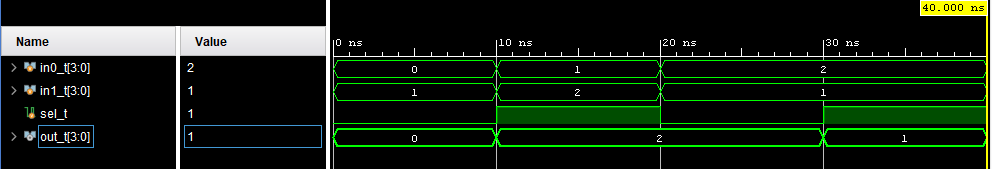
\includegraphics[width=1.0\textwidth]{MUX2_4B_TEST}
	\caption{MUX2-4B simulation waveform and ERT}
	\label{fig:sim_with_table}
\end{figure}

\begin{figure}[ht]\centering
	\begin{tabular}{l|rrrrrrrrrrrrrrrr}
		Time (ns): & 0 & 10 & 20 & 30 & 40 & 50 & 60 & 70 & 80 & 90 & 100 & 110 & 120 & 130 & 140 & 150 \\
		\midrule 
		Input num (hex) & 0 & 1 & 2 & 3 & 4 & 5 & 6 & 7 & 8 & 9 & a & b & c & d & e & f \\
		
		\bottomrule
		Output sseg (hex) & 40 & 79 & 24 & 30 & 19 & 12 & 02 & 38 & 00 & 10 & 08 & 03 & 46 & 21 & 06 & 0e \\
	\end{tabular}\medskip
	
	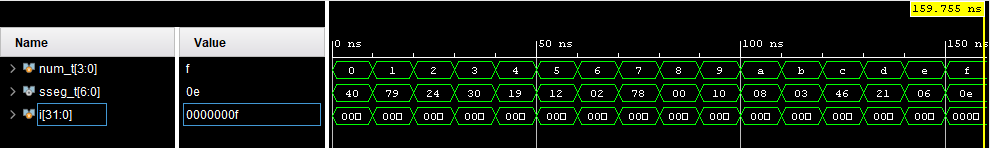
\includegraphics[width=1.0\textwidth]{decodertest}
	\caption{sseg- Decoder simulation waveform and ERT}
	\label{fig:sim_with_table}
\end{figure}
\clearpage

\begin{figure}[ht]\centering
	\begin{tabular}{l|rrrrrrrrrrrrrrrrr}
		Time (ns): & 0 & 10 & 20 & 30 & 40 & 50 & 60 & 70 & 80 & 90 & 100 & 110 & 120 & 130 & 140 & 150 & 160 \\
		\midrule 
		Input sw [7:0] (hex) & 0 & 1 & 1 & 21 & 21 & c8 & c8 & D3 & D3 & 3D & 3D & F0 & F0 & 0F & 0F & A5 & A5 \\
		
		Input sw [15] (hex) & 0 & 0 & 1 & 0 & 1 & 0 & 1 & 0 & 1 & 0 & 1 & 0 & 1 & 0 & 1 & 0 & 1  \\
		
		\bottomrule
		Output sseg & 40 & 79 & 40 & 79 & 08 & 00 & 08 & 03 & 21 & 21 & 0e & 40 & 78 & 78 & 12 & 12 & 00 \\
	\end{tabular}\medskip
	
	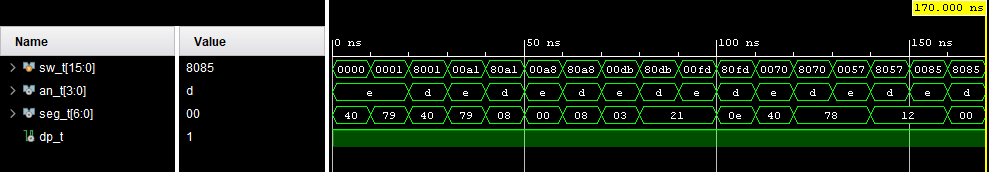
\includegraphics[width=1.0\textwidth]{toplevelmodfixed}
	\caption{sseg1 simulation waveform and ERT}
	\label{fig:sim_with_table}
\end{figure}


\begin{figure}[ht]\centering
	
	\includegraphics[width=1.0\textwidth]{f}
	\caption{Seven Segment display on right}
	\label{fig:sim_with_table}
\end{figure}
\clearpage

\begin{figure}[ht]\centering
	
	\includegraphics[width=1.0\textwidth]{c}
	\caption{Seven Segment display on left}
	\label{fig:sim_with_table}
\end{figure}
\clearpage


\section*{Code}

\begin{lstlisting}[style=Verilog,caption=mux2-4b Module Code,label=code:ex ]

// Ashlie Lackey and Chris Jones , ELC 2137, 2020 -2-26

module mux2_4b(

input [3:0]in0,

input [3:0]in1,

input sel,

output [3:0]out 

);



assign out = sel?in1:in0;

endmodule

\end{lstlisting}



\begin{lstlisting}[style=Verilog,caption=MUX Testbench Code,label=code:ex ]

// Ashlie Lackey and Chris Jones , ELC 2137, 2020 -2-26

module mux2_4b_test();

reg [3:0]in0_t, in1_t;

reg sel_t;

wire [3:0]out_t;



mux2_4b Mux(.in1(in1_t), .in0(in0_t), .sel(sel_t), .out(out_t));



initial begin

in0_t = 4'b0000;

in1_t = 4'b0001;

sel_t = 0;

#10;



in0_t = 4'b0001;

in1_t = 4'b0010;

sel_t = 1;

#10;



in0_t = 4'b0010;

in1_t = 4'b0001;

sel_t = 0;

#10;



in0_t = 4'b0010;

in1_t = 4'b0001;

sel_t = 1;

#10;



$finish ;

end

endmodule   //mux2_4b_test



\end{lstlisting}



\begin{lstlisting}[style=Verilog,caption=sseg Decoder Module Code,label=code:ex ]

// Ashlie Lackey and Chris Jones , ELC 2137, 2020 -2-26

module sseg_decoder (

input [3:0] num,

output reg [6:0] sseg

) ;

// 4 - bit to 7 - segment decode logic

// ( note : output is active low)

always @*

case (num) 

4'h0 : sseg = 7'b1000000 ;



4'h1 : sseg = 7'b1111001 ;



4'h2 : sseg = 7'b0100100 ;



4'h3 : sseg = 7'b0110000 ;



4'h4 : sseg = 7'b0011001 ;



4'h5 : sseg = 7'b0010010 ;



4'h6 : sseg = 7'b0000010 ;



4'h7 : sseg = 7'b1111000 ;



4'h8 : sseg = 7'b0000000 ;



4'h9 : sseg = 7'b0010000 ;



4'hA : sseg = 7'b0001000 ;



4'hB : sseg = 7'b0000011 ;



4'hC : sseg = 7'b1000110 ;



4'hD : sseg = 7'b0100001 ;



4'hE : sseg = 7'b0000110 ;



4'hF : sseg = 7'b0001110 ;

endcase

endmodule

\end{lstlisting}



\begin{lstlisting}[style=Verilog,caption=sseg Decoder Testbench Code,label=code:ex ]

// Ashlie Lackey and Chris Jones , ELC 2137, 2020 -2-26

module sseg_decoder_test () ;

reg [3:0]num_t;

wire [6:0]sseg_t;

integer i ; // Declare loop variable



sseg_decoder Bobby (.num(num_t), .sseg(sseg_t));



initial begin

for ( i =0; i <=8'hF ; i = i +1) begin

num_t = i;

#10;

end

$finish ;

end

endmodule // sseg_decoder_test

\end{lstlisting}



\begin{lstlisting}[style=Verilog,caption=Top-level Module Code,label=code:ex ]

// Ashlie Lackey and Chris Jones , ELC 2137, 2020 -2-26

module sseg1(

input [15:0]sw,

output [3:0]an,

output [6:0]seg,

output dp

);

wire [3:0] keith;

assign an[1] = ~sw[15];

assign an[0] = sw[15];

assign an[3:2] = 2'b11;

assign dp = 1;

mux2_4b william (.in1(sw[7:4]), .in0(sw[3:0]), .sel(sw[15]), .out(keith));

sseg_decoder robert(.num(keith), .sseg(seg));

endmodule

\end{lstlisting}



\begin{lstlisting}[style=Verilog,caption=Top Level Module Testbench Code,label=code:ex ]

// Ashlie Lackey and Chris Jones , ELC 2137, 2020 -2-26

module sseg1_test();

reg [15:0] sw_t;

wire [3:0] an_t;

wire [6:0] seg_t;

wire dp_t;

sseg1 sally(.sw(sw_t),.an(an_t),.seg(seg_t),.dp(dp_t)

);



initial begin

// Initialize

sw_t = 16'h0000; #10;

// Test case 1

sw_t [7:0] = 00000001;

sw_t [15] = 1'b0 ; #10;

sw_t [15] = 1'b1 ; #10;

// Test case 2

sw_t [7:0] = 00100001;

sw_t [15] = 1'b0 ; #10;

sw_t [15] = 1'b1 ; #10;

// Test case 3

sw_t [7:0] = 11001000;

sw_t [15] = 1'b0 ; #10;

sw_t [15] = 1'b1 ; #10;

// Test case 4

sw_t [7:0] = 11010011;

sw_t [15] = 1'b0 ; #10;

sw_t [15] = 1'b1 ; #10;

// Test case 5

sw_t [7:0] = 00111101;

sw_t [15] = 1'b0 ; #10;

sw_t [15] = 1'b1 ; #10;

// Test case 6

sw_t [7:0] = 11110000;

sw_t [15] = 1'b0 ; #10;

sw_t [15] = 1'b1 ; #10;

// Test case 7

sw_t [7:0] = 00001111;

sw_t [15] = 1'b0 ; #10;

sw_t [15] = 1'b1 ; #10;

// Test case 8

sw_t [7:0] = 10100101;

sw_t [15] = 1'b0 ; #10;

sw_t [15] = 1'b1 ; #10;

$finish;

end



endmodule

\end{lstlisting}





\end{document}

